\vspace{1cm}
{\small%
\section{Zwei und Mehrtore}
\subsection{Komplexe Wellenamplituden}
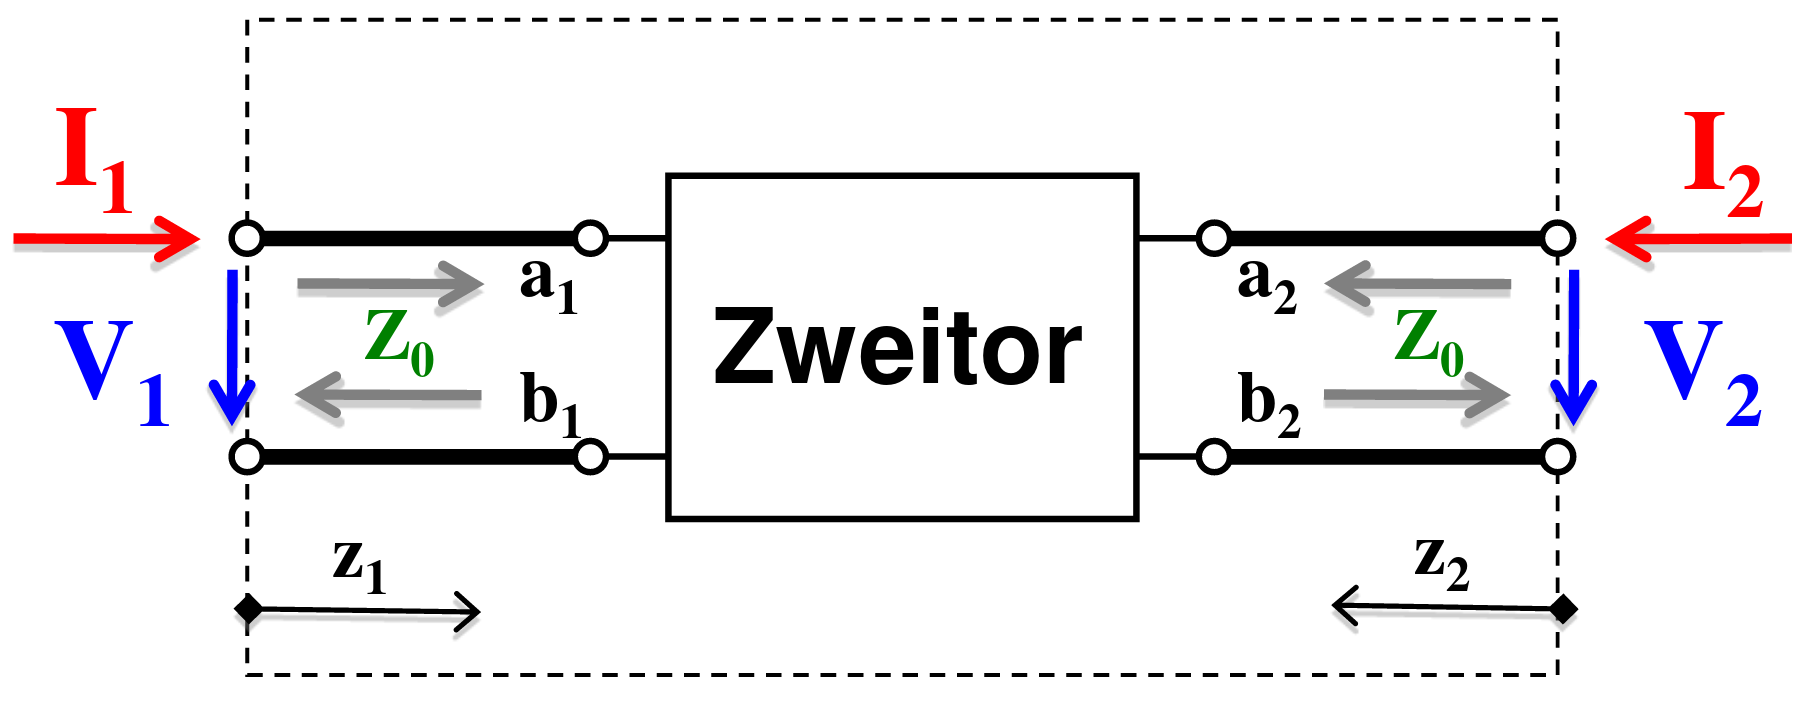
\includegraphics[width= 0.35\paperheight]{content/fuw/pictures/hf_zweitor.png}
    \begin{itemize}
        \itemsep0pt
        \item Verwendung von Strom/Spannung wenig sinnvoll, wegen der starken Empfindlichkeit zur Leitungslänge
        \item \textit{Stattdessen:} komplexe Amplituden $a$ und $b$
        \item Hinlaufende Welle $a_1$ bzw. $a_2$
        \item Rücklaufende Welle $b_1$ bzw. $b_2$
        \item Definition der Wellenamplituden:
        \begin{align*}
            a_k  = \dfrac{1}{2\sqrt{2 Z_0}}(U_k + Z_0 I_k)\\
            b_k  = \dfrac{1}{2\sqrt{2 Z_0}}(U_k - Z_0 I_k)
        \end{align*}
\end{itemize}
\subsection{Streuparameter}
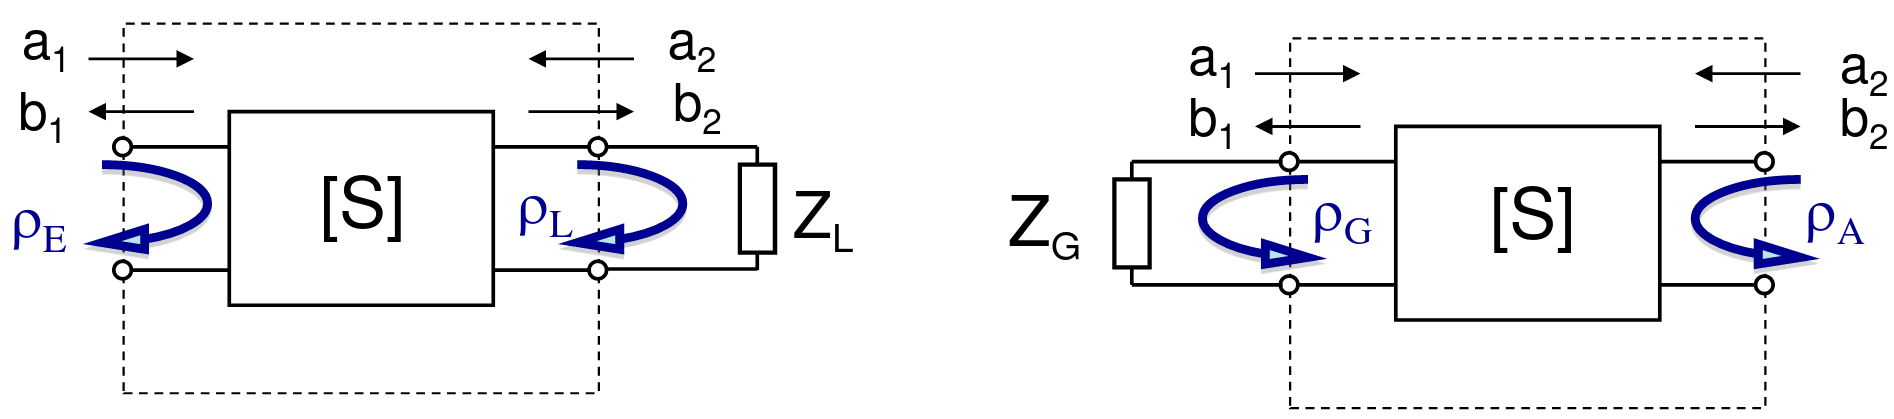
\includegraphics[width=0.35\paperheight]{content/fuw/pictures/hf_zweitor_reflektion.png}
\begin{itemize}
    \itemsep0pt
    \item Streuparameter der $S$-Matrix
    \item \textit{Allgemein:} \(\underline{b} = S \underline{a}\)
    \item Für ein Zweitor:
    \begin{align*}
        b_1 &= S_{11} a_1 + S_{12} a_2\\
        b_2 &= S_{21} a_1 + S_{22} a_2
    \end{align*}
    \item \textbf{Anpassung:} allseits reflexionsfrei\\
        \(s_{ii} = 0, \;\forall i \in (1;\; \mathrm{dim}(S))\)
    \item Eingangsreflexionsfaktor\\
        \(\rho_E = \dfrac{b_1}{a_1}; \;\;\; \rho_L = \dfrac{a_2}{b_2}\)
    \item Ausgangsreflexionsfaktor\\
        \(\rho_A = \dfrac{b_2}{a_2}; \;\;\; \rho_G = \dfrac{a_1}{b_1}\)
        \begin{align*}
            |\rho_E| = \left|S_{11} + \dfrac{S_{21} S_{12} \rho_L}{1 - S_{22} \rho_L}\right|\\
            |\rho_A| = \left|S_{22} + \dfrac{S_{12} S_{21} \rho_G}{1 - S_{11} \rho_G}\right|
        \end{align*}
    \item \textbf{Reziprozität} (Übertragungssymmetrie): \(S = S^\top\)
    \item \textbf{Verlustfreie} n-Tore ($S$ unitär):\\
        \(\sum^n_{i=1} |b_i|^2 = \sum^n_{i=1} |a_i|^2 \implies S^\top S^* = I\)
    \item Verlustfreies, reziprokes, allseits angepasstes 3-Tor\\
        \(\implies\) nicht realisierbar
\end{itemize}
\subsection{Alternative Netzwerkdarstellungen}
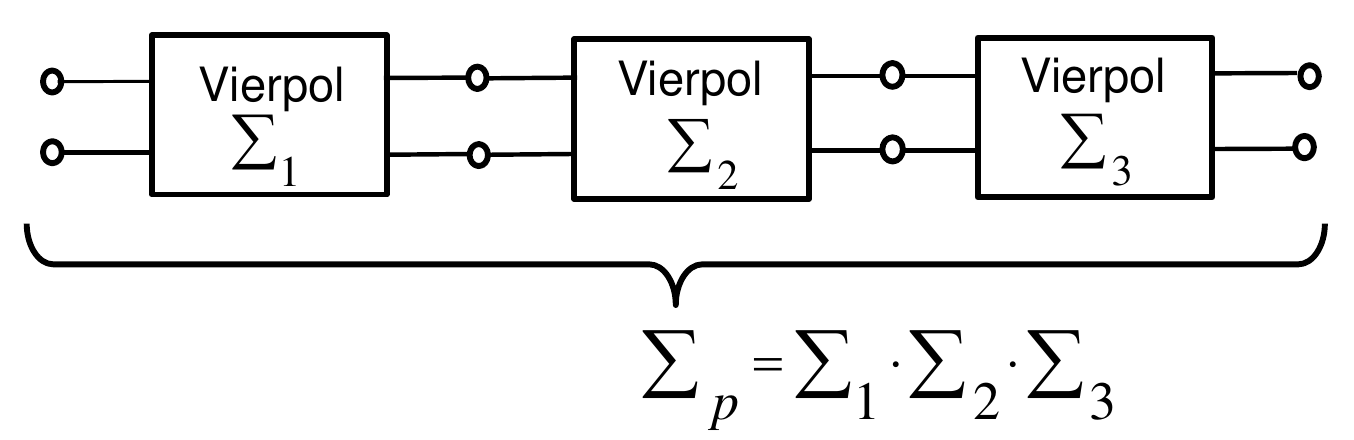
\includegraphics[width=0.35\paperheight]{content/fuw/pictures/fuw_transmissionsmatrix.png}
\begin{itemize}
    \itemsep0pt
    \item \textbf{Wellentransmissionsmatrix} $\Sigma$:\\
        \[\begin{bmatrix}b_1\\ a_1\end{bmatrix} = \begin{bmatrix}\Sigma_{11} & \Sigma_{12}\\ \Sigma_{21} & \Sigma_{22}\end{bmatrix} \begin{bmatrix}a_2\\ b_2\end{bmatrix}\]\\
    \item Streumatrix $\to$ Transmissionsmatrix
        \begin{align*}
            \Sigma_{11} &= -\dfrac{\Delta_S}{S_{21}} &\Sigma_{12} = \dfrac{S_{11}}{S_{21}}\\
            \Sigma_{21} &= -\dfrac{S_{22}}{S_{21}} &\Sigma_{22} = \dfrac{1}{S_{21}}
        \end{align*}
    \item \textbf{Ketten- bzw. ABCD-Matrix}:
        \[\begin{bmatrix}u_1\\ i_1\end{bmatrix} = \begin{bmatrix}A & B\\ C & D\end{bmatrix} \begin{bmatrix}u_2\\ -i_2\end{bmatrix}\]
        \item  $u$ und $i$ sind normierte Spannungen und Ströme:\\
            \(u = \dfrac{U}{\sqrt{Z_0}}; \;\; i = I\sqrt{Z_0}\)
        \item ABCD $\to$ Streumatrix:
            \begin{align*}
                S_{11} &= \dfrac{A+B-C-D}{A+B+C+D}, &S_{12} = \dfrac{2\:\mathrm{det}(ABCD)}{A+B+C+D},\\
                S_{21} &= \dfrac{2}{A+B+C+D}, &S_{22} = \dfrac{-A+B-C+D}{A+B+C+D}
            \end{align*}
        \item Streumatrix $\to$ ABCD:
            \begin{align*}
                A &= \dfrac{-\Delta_S + S_{11} - S_{22} + 1}{2 S_{21}},\\
                B &= \dfrac{\Delta_S + S_{11} + S_{22} + 1}{A+B+C+D},\\
                C &= \dfrac{\Delta_S - S_{11} - S_{22} + 1}{2 S_{21}},\\
                D &= \dfrac{-\Delta_S - S_{11} S_{22} + 1}{2 S_{21}}
            \end{align*}
        \item Längwiderstand bzw. Querleitwert mit Bezugswiderstand $Z_0$:\\
            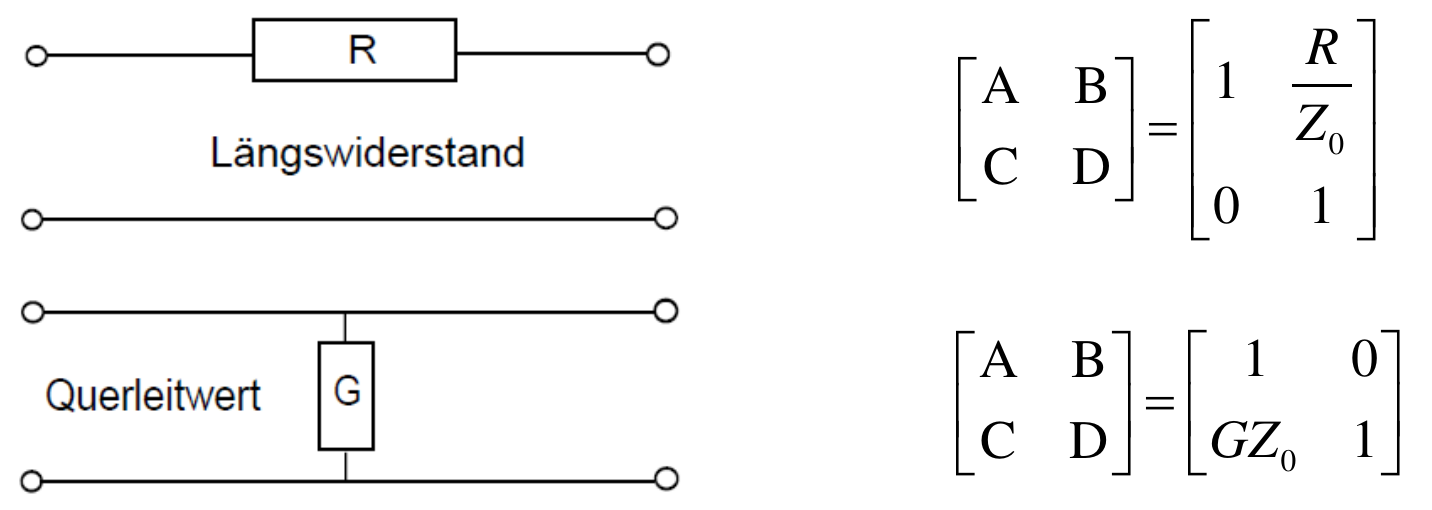
\includegraphics[width=0.35\paperheight]{content/fuw/pictures/fuw_kettenmatrix_widerstand_leitwert.png}
        \item Verlustlose Leitung (Wellenwiderstand $Z_l$, elektrische Länge $\beta l$, geometrische Länge $l$):
                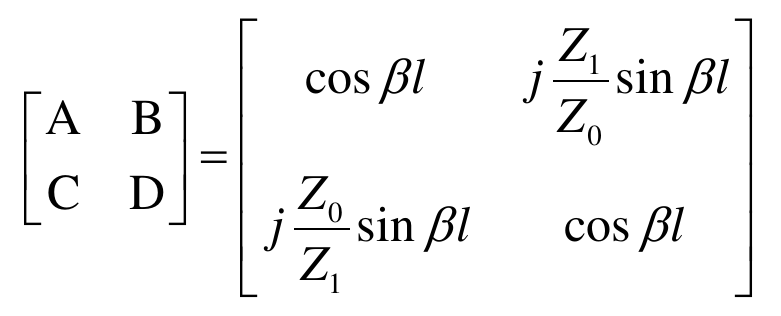
\includegraphics[width=0.28\paperheight]{content/fuw/pictures/fuw_kettenmatrix_leitung.png}
\end{itemize}
\subsection{Betriebsverhalten von Zweitoren}
\subsubsection{Zweitorverstärkung}
\begin{itemize}
    \itemsep2pt
    \item Die Übertragungsleistungsverstärkung (Gewinn $G$) ist die Ausgangsleistung bezogen auf die verfügbare Generatorleistung
    \item \(G = \dfrac{1 - |\rho_G|^2}{|1 - \rho_G \rho_E|^2} \cdot |s_{21}|^2 \cdot \dfrac{1 - |\rho_L|^2}{|1 - \rho_{L}s_{22}|^2}\)
    \item Bei Rückwirkungsfreiheit $s_{12} = 0$ ($\rho_E = s_{11}$):\\
        \(G = \dfrac{1 - |\rho_G|^2}{|1 - \rho_G s_{11}|^2} \cdot |s_{21}|^2 \cdot \dfrac{1 - |\rho_L|^2}{|1 - \rho_{L}s_{22}|^2}\)
    \item \textit{Daumenregel für Rückwirkungsfreiheit}:\\
        \(\dfrac{S_{12}}{S_{21}} \ll 1 \implies \dfrac{S_{12}}{S_{21}} \leq 0.1\)
    \item Maximale (unilaterale für $s_{12} = 0$) Leistungsverstärkung:\\
        \(G_{max} = \dfrac{|s_{21}^2|}{(1 - |s_{11}|^2) (1 - |s_{22}^2|)}\)
\end{itemize}
\subsubsection{Verstärker mit Anpassnetzwerken}
\begin{itemize}
    \itemsep0pt
    \item Max. Leistungsverstärkung erfordert Wirkleistungsanpassung am Ein- und Ausgang
    \item Hochfrequenzverstärker (Transistoren) weisen stark reaktive u. frequenzveränderliche Impedanz auf
    \item Diese muss durch geeignete reaktive Netzwerke angepasst werden
    \item Probleme:
        \begin{itemize}
            \itemsep0pt
            \item Reaktive Anpassung $\to$ schmalbandig
            \item Reflexionen zwischen Verstärker und Anpassnetzwerk $\to$ Stabilitätsprobleme
        \end{itemize}
    \item \textbf{Absolute Stablilität:} Die Tore verhalten sich, unabhängig von der Beschaltung, \textit{passiv} $\implies$ \(\left(\mathrm{Re}\{Z_E\} > 0\right) \:\wedge\: \left(\mathrm{Re}\{Z_A\} > 0\right)\)
    \item \textbf{Bedingungen für Absolute Stabilität}:
    \begin{align*}
        &|S_{11}| < 1, &|S_{12} \cdot S_{21}| < 1 - |S_{22}|^2,\\
        &|S_{22}| < 1, &|S_{12} \cdot S_{21}| < 1 - |S_{11}|^2,\\
        %&K > 1; &K = \dfrac{1 + |\Delta_S|^2 - |S_{11}|^2 - |S_{22}|^2}{|2\, S_{12} S_{21}|}
    \end{align*}
        \(K = \dfrac{1 + |\Delta_S|^2 - |S_{11}|^2 - |S_{22}|^2}{|2\, S_{12} S_{21}|} > 1\)
    \item \textbf{Stabilitätskreise} für den Ein- ($C_L$, $R_L$) bzw Ausgang ($C_G$, $R_G$):
        \begin{align*}
            &C_L = \dfrac{\left(S_{22} - \Delta_S S_{11}^*\right)^*}{|S_{22}|^2 - |\Delta_S|^2},\
            &R_L = \left|\dfrac{S_{12} S_{21}}{|S_{22}|^2 - |\Delta_S|^2}\right|,\\
            &C_G = \dfrac{\left(S_{11} - \Delta_S S_{22}^*\right)^*}{|S_{11}|^2 - |\Delta_S|^2},\
            &R_G = \left|\dfrac{S_{12} S_{21}}{|S_{11}|^2 - |\Delta_S|^2}\right|,
        \end{align*}
\end{itemize}
\subsection{Gebräuchliche Mehrtorschaltungen}
\subsubsection{Leitungskoppler, Reflektometerschaltung}
\begin{minipage}{.4\paperheight}
    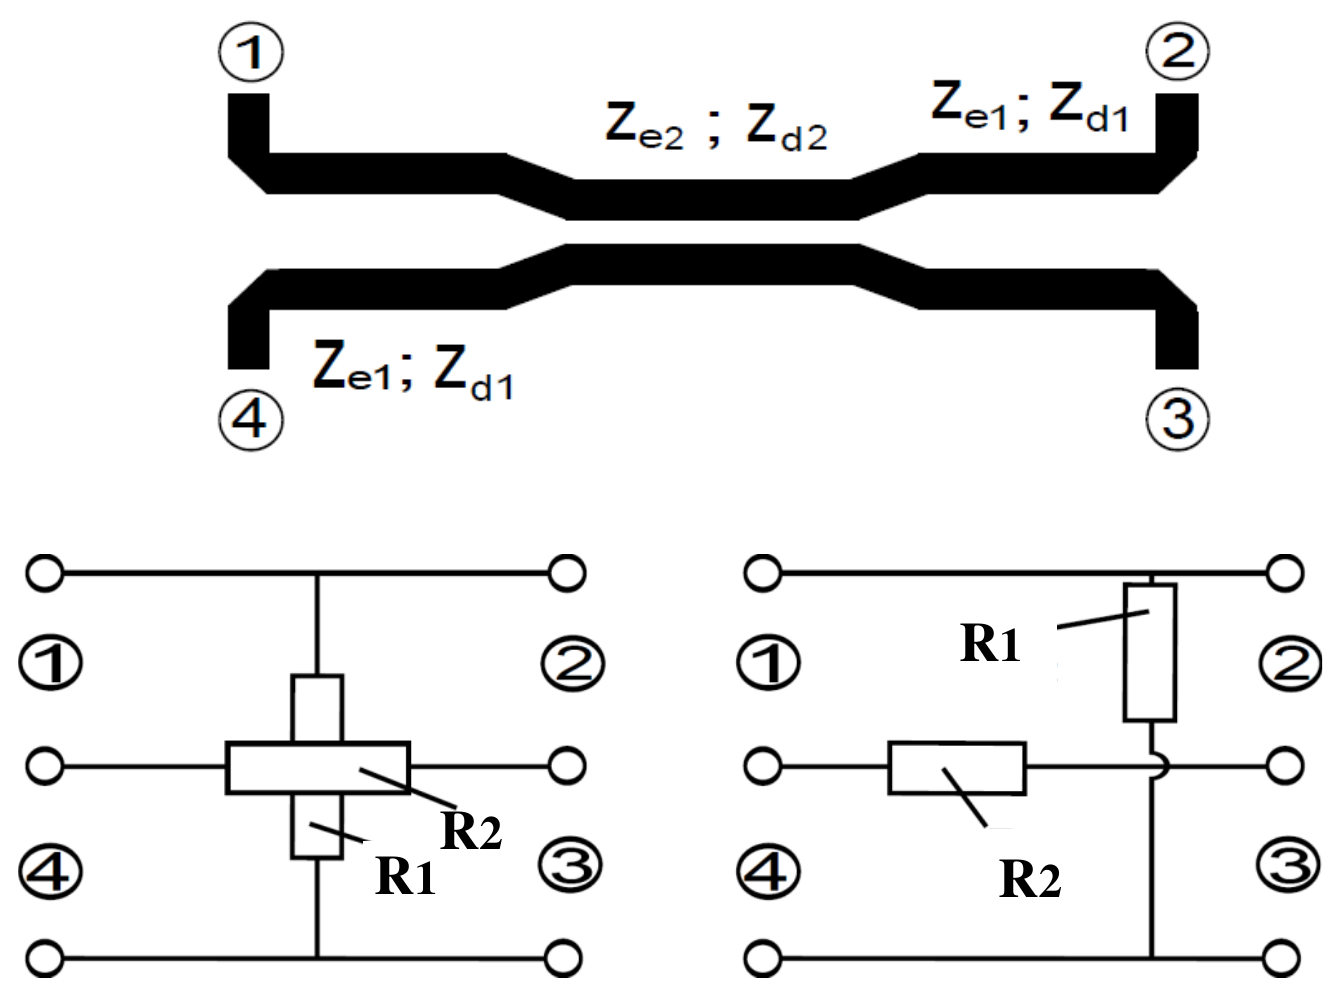
\includegraphics[width=.12\paperheight]{content/fuw/pictures/fuw_leitungs_und_resistive_koppler.png}
    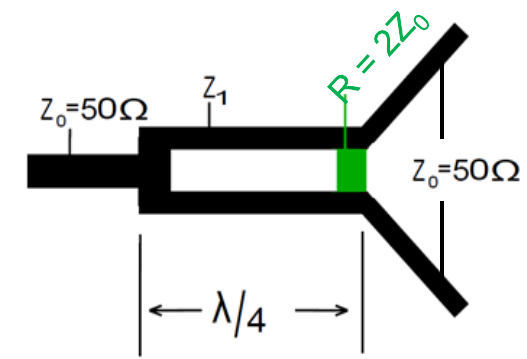
\includegraphics[width=.12\paperheight]{content/fuw/pictures/fuw_wilkinsonteiler1.png}
    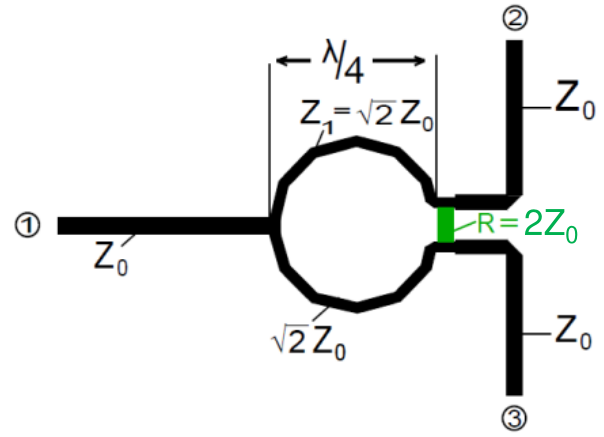
\includegraphics[width=.12\paperheight]{content/fuw/pictures/fuw_wilkinsonteiler2.png}
\end{minipage}
\begin{itemize}
    \itemsep0pt
    \item Dienen dazu hin- und rücklaufenden Wellen a \& b zu trennen
    \item \textbf{Bauelemente zur Trennung der Welle:} \textit{Richtkoppler}
    \item Typische Koppler:
        \begin{itemize}
            \itemsep0pt
            \item Leitungskoppler
            \item Resistive Koppler
            \item Transformatorkoppler
            \item Null-Grad-Koppler bzw. Signalteiler mit $\lambda/4$-Leitungen
        \end{itemize}
\end{itemize}
}
